\documentclass[11pt,a4paper,titlepage]{article}
\usepackage[english, ngerman]{babel}
%\usepackage{bibgerm} % Zum Einbinden einer Bibliothek (wird hier nicht benötigt)
\usepackage[latin1]{inputenc}
\usepackage{graphicx}
\usepackage{epstopdf} % wandelt automatisch eps- in pdf-Dateien um, falls pdf als Ausgabeformat gewählt wird
\usepackage{include/IHA_listing} % einbinden von Quellcode
\setupListingMatlab % lade Setup für Matlab Quellcode, Parameter können in der *.sty file geändert werden ;)
\usepackage[top=3cm, bottom=2.7cm, left=3cm, right=3cm]{geometry} % Package zum einfachen Einstellen des Seitenlayouts
\usepackage{amsmath} % Package zum Einbinden von Formeln etc.
\usepackage{subfigure}
\usepackage{placeins}
\usepackage{latexsym}
\usepackage{amsfonts}
\usepackage{amssymb}	
\usepackage{fancyhdr}
\usepackage{lastpage}
\usepackage[ngerman, num]{isodate}
\usepackage{marvosym}
\usepackage{eurosym}
\usepackage{url}
\usepackage{wrapfig}
\usepackage{xcolor}
\usepackage{tcolorbox}
\usepackage{hyperref}
\parindent0mm
\usepackage[protrusion=true,expansion=true]{microtype}
%\usepackage[final]{microtype}
%\usepackage{fontspec}
\usepackage{cmbright}

\newcommand{\titleFull}{IHAB-rl Mobile Software\\\vspace{0.5cm}Standalone}
\renewcommand{\title}{IHAB-rl Mobile Software}
\newcommand{\Institute}{Institute of Hearing Technology and Audiology, Oldenburg}
\newcommand{\version}{v1.3}
%
\pagestyle{fancy}
\lhead{\footnotesize \parbox{11cm}{\Institute} }
\rhead{\footnotesize \sffamily \title\ \thepage\ / \pageref{LastPage}}
\lfoot{\footnotesize \parbox{11cm}{Contact: \Letter\ ulrik.kowalk@jade-hs.de} }
\cfoot{}
\rfoot{\footnotesize \sffamily \title\ \thepage\ / \pageref{LastPage}}
\renewcommand{\footrulewidth}{0.4pt}

%
\begin{document} 
 \selectlanguage{english}
\pagestyle{empty}

\sffamily
\mdseries


\textcolor[rgb]{1,1,1}{.}
	\vspace{3cm}
	\begin{center}
	
	\begin{figure}[h]
		\centering
			
\includegraphics[width=0.30\textwidth]{images/Logo_shadow.jpg}
		\label{fig:Fahrplan}
	\end{figure}
	\vspace{3cm}
	\Huge
	\titleFull \ \version
	\normalsize
	\\
	\vspace{1cm}
	Documentation\\
	\vspace{1cm}
	Last updated: \today\\
	\vspace{1cm}
	Source: \url{https://github.com/IHAB-RL/IHAB_MobileSoftware.git}
	\vfill
	\end{center}

%
%\cfoot{}
\clearpage

\tableofcontents

\clearpage

\setcounter{page}{1}
\pagestyle{fancy}

\section{Introduction}

The application you have obtained is a \textbf{standalone} derivative of the bluetooth system. No additional equipment is therefore required except for a computer to facilitate installation and data transfer. The software has been tested on the following devices:
\begin{itemize}
	\item LG Electronics Nexus 5 (Android 5.1 \& 6.0.1)
	\item Motorola XT1032 (Androd 5.1)
	\item Motorola Moto G2  (Android 6.0)
	\item Lenovo TB2 X30F (Android 6.0.1)
\end{itemize}

This software is still in development. Please feel free to contact us in case of any bugs or difficulties occurring during installation and usage.

\section{Installation}

\subsection{Requirements}

The device should be reset to its operating system default (\textit{Settings}$\rightarrow$\textit{Backup\&reset}$\rightarrow$\textit{Factory data reset}) prior to the installation. All accounts (\textit{Settings}$\rightarrow$\textit{Accounts}) as well as device administrators (\textit{Settings}$\rightarrow$\textit{Security}$\rightarrow$\textit{Device administrators}) need to be removed, too. On an average size display, the font size should be set to \textit{Large} (\textit{Settings}$\rightarrow$\textit{Display}$\rightarrow$\textit{Font size}). Required for the installation are:

\begin{itemize}
	\item USB connection between smartphone and computer
	\item Free software \textit{ADB} (Android Debug Bridge), e.g. ``Minimal ADB and Fastboot''
	\item IHAB mobile .apk installation file
	\item Questionnaire .xml file
	\item helpful: free Android file manager, e.g. \href{https://total-commander.de.uptodown.com/android}{``Total Commander''}
\end{itemize}


\subsection{Installation steps}

\begin{enumerate}

	\item Install ADB on the computer and add it to the system path
	\item Enable the developer options on the smartphone. How to do this might vary from model to model. The usual procedure is by opening \textit{Settings$\rightarrow$About phone}. At the bottom is an entry showing the \textit{Build number}. This needs to be clicked 7 times until a message appears.
	\item Go to \textit{Settings}$\rightarrow$\textit{Developer options} and enable \textit{USB Debugging}.
	\item Connect the phone to the computer and allow debugging via the dialogue on the phone.
	\item The next step is to establish a working connection between the smartphone and the computer. In order to check for a connection, open a console and type in ``\texttt{adb devices}''. If everything is okay, ADB should find a device. If not, check your connection. In case the computer does not understand the command, ADB needs to be added to the system path.
	\item Now that a connection has been verified, move the console to the directory that holds the .apk file and input ``\texttt{adb install IHAB\_Mobile\_Standalone.apk}''. This should copy and install the application. 
	\item After the installation is complete, input ``\texttt{adb shell dpm set-device-owner \newline com.fragtest.android.pa/.AdminReceiver}''. This makes the application a device owner, which is needed for it to run as a dedicated device.
	\item Now input ``\texttt{adb shell appops set android TOAST\_WINDOW deny}'' to keep any information from popping up and confusing the user.
	\item Opening the application will throw an error because no questionnaire file is present (however, this step is necessary to build the file system). Using the Windows Explorer, copy your questionnaire file to the \textit{quest} folder within the application directory (\textit{IHAB}). Depending on the device it might be necessary to enable the data transfer protocol MTP on the phone. A downward swipe starting from the top of the display shows the USB protocol which can then be altered. Alternatively you can enter the command ``\texttt{adb push [questionnaire file name] sdcard/ihab/quest}''.
	\item Restart the phone by entering ``\texttt{adb restart}''.
\end{enumerate}


\section{Usage of the application}\label{sec_usage}

\begin{wrapfigure}{r}{5cm}
\vspace{-0.5cm}
		\centering
\fbox{\begin{minipage}{0.30\textwidth}
			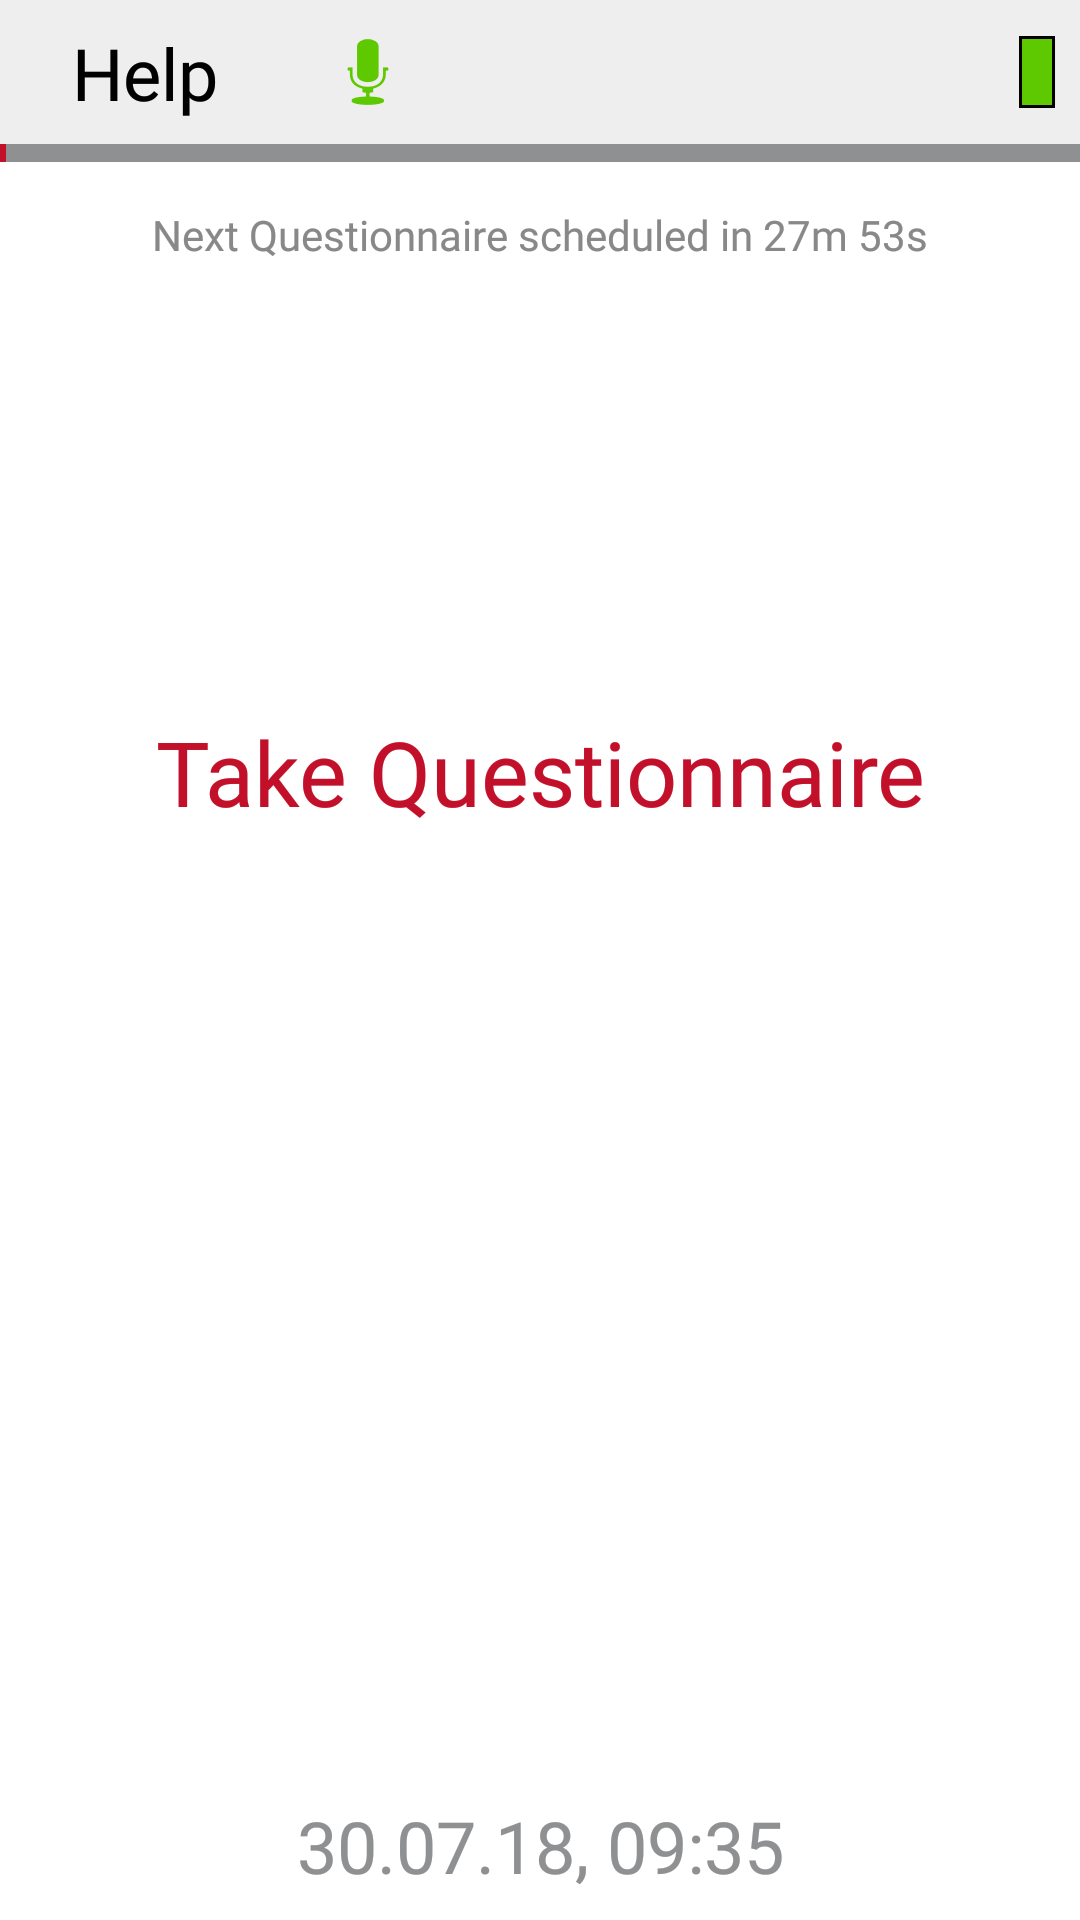
\includegraphics[width=1.00\textwidth]{images/Screenshot_2018-07-30-09-35-59.png}
			\label{fig:menu}
			\end{minipage}}
	\end{wrapfigure}

If the installation was successful, the smartphone runs as a dedicated device (or kiosk device), meaning that the user cannot leave the application or make alterations to the operating system. Most buttons are disabled or limited to specific use -- including the power button which will only restart the device after a long push.\\
\\
The menu view (see figure on the right) of the application features a bar at the top with a \textit{Help} button, providing a general explanation of the main answer formats. Next to it is a microphone symbol that can change its color according to whether a wireless connection has been established (green), no connection can be made (gray) or -- in this case -- standalone mode (blue). On the right hand side is a battery symbol displaying the current state of charge.\\
\\
The center of the screen features the "Take Questionnaire" button (in case of no major errors present) which can be used to manually start a questionnaire at any given time. Above it is a display of the time until the next questionnaire is triggered. If a questionnaire is prompted the font size increases, accompanied by vibrating alert.\\

\section{Developer Mode}\label{sub:developer}

When testing a new questionnaire, it is helpful to disable the KIOSK mode. The easiest way is the \textit{Developer mode}, which can be unlocked by copying a specific file to the main application folder (\textit{IHAB}). The file may be empty and must be named ``config'' without a formatted ending. On the next start the application will boot into developer mode, which also grants access to the preferences menu (although this mostly concerns the bluetooth version). The action can be reversed by simply deleting the file from the folder.

\section{Compilation of a questionnaire}

The questionnaires are generated on the basis of .xml files which can be altered to suit the needs of the experiment. Generally it is a good idea to start from an existing file and make changes, testing them regularly on the smartphone in order to guarantee errorless functionality. In case of formal mistakes (e.g. missing brackets or typos within tags) the application might crash. 

\subsection{Location of questionnaire files}

Questionnaire files are placed in the \textit{quest} folder located in the application directory. The application will automatically sort all questionnaire files alphabetically and pick the uppermost. If you like to use a different questionnaire, you can choose manually from the preferences menu (see \ref{sub:developer}), but we recommend placing only a single file in the \textit{quest} folder in order to avoid confusion. 

\subsection{Head}

The head consists of two lines that must not be changed, but may become obsolete in future releases.

\subsection{Timer} 





Two different timer settings exist: \textit{interval} and \textit{fixed schedule}. When choosing interval, a \texttt{mean} and \texttt{deviation} tag and value can be set. The application generates a random interval true to a uniform distribution within the given limits (mean$\pm$deviation). This can be beneficial in order to avoid sampling artifacts, e.g. suggesting a questionnaire every 60 minutes to someone who is always listening to the news at that time. If the scheduling interval should not be random, a deviation value of "0" is set. The timer is re-initiated after a questionnaire has been finalized.
%
\begin{center}
\begin{tcolorbox}[colback=black!10!white,colframe=black!50!white]
\texttt{<timer mean="1800" deviation="300"></timer>}
\end{tcolorbox}
\end{center}
%
If it is desired to suggest a questionnaire at specific times, the \texttt{date} tag must be set. The value is entered in form of a String, meaning a time within quotation marks, e.g. "13:47". The system uses the 24h format HH:MM and multiple entries can be entered by concatenating times with a semicolon, e.g. "12:15;17:21;14:41". Times are sorted automatically by the application. 
%
\begin{center}
\begin{tcolorbox}[colback=black!10!white,colframe=black!50!white]
\texttt{<timer date="12:15;13:13;14:41;17:21;8:10;08:12"></timer>}
\end{tcolorbox}
\end{center}

\subsection{Title}

The title tag can be set to personal taste and is formally needed but does not appear in the output result files.
%
\begin{center}
\begin{tcolorbox}[colback=black!10!white,colframe=black!50!white]
\texttt{<title>\\
\hspace*{0.5cm}<text>Exemplary Questionnaire</text>\\
</title>}
\end{tcolorbox}
\end{center}

\subsection{Questions}

A question consists of an opening \texttt{question} tag including some properties, e.g. id, type, and filter. Then follows the label -- the actual question. After that comes a suite of answer options, which are defined by a unique \texttt{option id}. Although there are no restrictions, it has proven useful in practice to combine \texttt{question id} and \# of the answer using an underscore (the underscore is omitted internally). Below is an example of a question with three answer options:
%
\begin{center}
\begin{tcolorbox}[colback=black!10!white,colframe=black!50!white]
\texttt{
$<$question id="10104" type="radio" filter="10103\_01"$>$\\
\hspace*{0.5cm}$<$label$>$\\
\hspace*{0.5cm}$<$text$>$What are you currently doing?$<$/text$>$\\
\hspace*{0.5cm}$<$/label$>$\\
\hspace*{0.5cm}$<$option id="10104\_01"$>$\\
\hspace*{1cm}$<$text$>$Relaxing$<$/text$>$\\
\hspace*{0.5cm}$<$/option$>$\\
\hspace*{0.5cm}$<$option id="10104\_02"$>$\\
\hspace*{1cm}$<$text$>$Eating$<$/text$>$\\
\hspace*{0.5cm}$<$/option$>$\\
\hspace*{0.5cm}$<$option id="10104\_03"$>$\\
\hspace*{1cm}$<$text$>$Paperwork$<$/text$>$\\
\hspace*{0.5cm}$<$/option$>$\\
$<$/question$>$}
\end{tcolorbox}
\end{center}
%
The \texttt{question id} serves as a unique question identifier, the \texttt{type} sets the answer format (see \ref{sub:format}) and the \texttt{filter} determines the conditions under which the question is included in the current sequence (see \ref{sub:logic}).


\subsection{Finish}

The last question must be the \texttt{finish} page which automatically includes a button that completes the questionnaire and saves the results:
%
\begin{center}
\begin{tcolorbox}[colback=black!10!white,colframe=black!50!white]
\texttt{
$<$finish$>$\\
\hspace*{0.5cm}$<$text$>$Thank you!$<$/text$>$\\
$<$/finish$>$}
\end{tcolorbox}
\end{center}

\subsection{Checkbox grouping and exclusivity}

If only one option out of a group of options might be logically possible (see exemplary options 1-3 below), they can form a \texttt{group}. If one item out of this group is selected, the others are automatically deselected. Multiple groups can exist within one question. An extreme form of this is the \texttt{exclusive} tag (option 5), which deselects every other item from the respective list of answers except itself and automatically deselects itself if another item is chosen.
%
\begin{center}
\begin{tcolorbox}[colback=black!10!white,colframe=black!50!white]
\texttt{
$<$question id="10111" type="checkbox"$>$\\
\hspace*{0.5cm}$<$label$>$\\
\hspace*{1cm}$<$text$>$Where does sound originate from?$<$/text$>$\\
\hspace*{0.5cm}$<$/label$>$\\
\hspace*{0.5cm}$<$option id="10111\_01" group="1"$>$\\
\hspace*{1cm}$<$text$>$Single person$<$/text$>$\\
\hspace*{0.5cm}$<$/option$>$\\
\hspace*{0.5cm}$<$option id="10111\_02" group="1"$>$\\
\hspace*{1cm}$<$text$>$2-3 persons$<$/text$>$\\
\hspace*{0.5cm}$<$/option$>$\\
\hspace*{0.5cm}$<$option id="10111\_03" group="1"$>$\\
\hspace*{1cm}$<$text$>$4 or more persons$<$/text$>$\\
\hspace*{0.5cm}$<$/option$>$\\
\hspace*{0.5cm}$<$option id="10111\_04"$>$\\
\hspace*{1cm}$<$text$>$Public announcement$<$/text$>$\\
\hspace*{0.5cm}$<$/option$>$\\
\hspace*{0.5cm}$<$option id="10111\_05" condition="exclusive"$>$\\
\hspace*{1cm}$<$text$>$It is quiet.$<$/text$>$\\
\hspace*{0.5cm}$<$/option$>$\\
$<$/question$>$}
\end{tcolorbox}
\end{center}

\subsection{Default items}

An item can be set as preselected default using the \texttt{default} tag instead of \texttt{option} as shown below:
%
\begin{center}
\begin{tcolorbox}[colback=black!10!white,colframe=black!50!white]
\texttt{
$<$default id="10109\_03"$>$\\
\hspace*{0.5cm}$<$text$>$Not much$<$/text$>$\\
$<$/default$>$}
\end{tcolorbox}
\end{center}

\subsection{Comments}

Two types of comments are supported by the questionnaire format. Single line comments start with ``//'', multiple line comments are parenthesized by ``\texttt{$/*$}'' and ``\texttt{$*/$}''.

\clearpage

\subsection{Answer formats}\label{sub:format}

The \texttt{type} of answer is set in the opening line of the \texttt{question} tag.\\
\\
Several answer formats have been implemented:
\begin{itemize}
	\item \texttt{radio}: multiple options, single choice
	\item \texttt{checkbox}: multiple options, multiple choice
	\item \texttt{emoji}: a scale of up to 5 emojis to assess personal feelings
	\item \texttt{text}: free text form
	\item \texttt{sliderFix}: slider with fixed scale and labels, result is answer ID
	\item \texttt{sliderFree}: slider with no scale but labels, result is normalized value
	\item \texttt{finish}: last question, including a ``Push to complete'' button
\end{itemize}

\subsection{Logic}\label{sub:logic}

In order to allow for high specificity and efficiency, questions can be equipped with logical decision parameters that establish whether or not a question will be included in the current suite. The switch is located in the opening line of each question under the tag \texttt{filter} in form of a comma-separated concatenation of all included conditions. Two scenarios exist: positive and negative. A question will only be included if \textbf{ALL} positive conditions are satisfied and it will not be included as long as at least \textbf{ONE} negative condition (indicated by a prefixed ``!'') is satisfied (e.g. \texttt{filter="10103\_02,10103\_05,!10111\_09"}). Think: positive - necessary criterion, negative -- sufficient criterion.\\
\\
The filter conditions are the option ID's of answer items from earlier questions of the current questionnaire session. Whenever an answer is chosen by the user, its ID is stored to memory and before a question is displayed, a filter checks whether given conditional ID's can be found in the memory.\\

\section{Data transfer}

For every questionnaire that has been answered, a resulting .xml file is produced which can be found in the \textit{data} folder within the application directory. In order to simplify data transfer we have developed a Matlab interface which can also be used to stop the application (because for safety reasons this is not provided or at least not trivial) and to erase all data from the device. The software is self-explanatory and can be found under GitHub: \url{https://github.com/IHAB-RL/IHAB_DataExtraction.git}. Please note that so far it has only been tested under Windows 7.

\clearpage

\section{License}

 Copyright 2018 \Institute\\
\\
   Licensed under the Apache License, Version 2.0 (the ``License'');
   you may not use this file except in compliance with the License.
   You may obtain a copy of the License at\\
\\
     \url{http://www.apache.org/licenses/LICENSE-2.0}\\
\\
   Unless required by applicable law or agreed to in writing, software
   distributed under the License is distributed on an ``AS IS'' BASIS,
   WITHOUT WARRANTIES OR CONDITIONS OF ANY KIND, either express or implied.
   See the License for the specific language governing permissions and
   limitations under the License.

\end{document} 